\documentclass{../CursoLaTeX}

\subtitle{Figuras}


\usepackage[export]{adjustbox}
\usepackage[brazilian]{babel}
\usepackage{subfigure}
\usepackage{hyperref}

\setbeamertemplate{caption}[numbered]
\graphicspath{{./figs/}{./figs/logos/}{./figs/formatos/}}


\begin{document}

%%%%%%%%%%%%%%%%%%%%%%%%%%%%%%%%%%%%%%%%%%%%%%%%%%%%%%%%%
\begin{frame}{Sumário} 
  \tableofcontents[] 
\end{frame}

%%%%%%%%%%%%%%%%%%%%%%%%%%%%%%%%%%%%%%%%%%%%%%%%%%%%%%%%%
\section{Pacote \textit{graphicx}}

%%%%%%%%%%%%%%%%%%%%%%%%%%%
\begin{frame}[fragile]{Pacote \textbf{graphicx}}
O pacote \textbf{graphicx} possibilita a inclusão de imagens através do comando \bs\textit{includegraphics}.
\lstset{language=Pascal}

\begin{lstlisting}[style=latex, linewidth=12cm, xleftmargin=2cm]
\documentclass{article}

% Pacotes
\usepackage{graphicx}

\begin{document}

  % Inserindo figura
  
\includegraphics{formas.png}

\end{document}
\end{lstlisting}

\end{frame}


%%%%%%%%%%%%%%%%%%%%%%%%%%%%%%%%%%%%%%%%%%%%%%%%%%%%%%%%%
\section{Layout}

%%%%%%%%%%%%%%%%%%%%%%%%%%%
\begin{frame}[fragile,t]{Figura Padrão} 
\framesubtitle{Comando \textit{includegraphics}}

\makebox[0.65\linewidth][l]{Código \LaTeX:}%
\makebox[0.35\linewidth][l]{Saída:}% 
\vfill
\begin{LTXexample}[style=example,width=0.35\linewidth]

\includegraphics{formas.png}
\end{LTXexample}
\end{frame}

%%%%%%%%%%%%%%%%%%%%%%%%%%%
\begin{frame}[fragile,t]{Redimensionamento}
\framesubtitle{Opção \textit{scale}}

\makebox[0.65\linewidth][l]{Código \LaTeX:}%
\makebox[0.35\linewidth][l]{Saída:}% 
\vfill
\begin{LTXexample}[style=example,width=0.35\linewidth]

\includegraphics[scale=0.5]{formas.png}
\end{LTXexample}
\end{frame}


%%%%%%%%%%%%%%%%%%%%%%%%%%%
\begin{frame}[fragile,t]{Redimensionamento por Comprimento}
\framesubtitle{Opção \textit{width}}

\makebox[0.65\linewidth][l]{Código \LaTeX:}%
\makebox[0.35\linewidth][l]{Saída:}% 
\vfill
\begin{LTXexample}[style=example,width=0.35\linewidth]

\includegraphics[width=\textwidth]
                  {formas.png}
\end{LTXexample}
\end{frame}

%%%%%%%%%%%%%%%%%%%%%%%%%%%
\begin{frame}[fragile,t]{Redimensionamento por Altura}
\framesubtitle{Opção \textit{height}}

\makebox[0.65\linewidth][l]{Código \LaTeX:}%
\makebox[0.35\linewidth][l]{Saída:}% 
\vfill
\begin{LTXexample}[style=example,width=0.35\linewidth]

\includegraphics[height=2cm]{formas.png}
\end{LTXexample}
\end{frame}

%%%%%%%%%%%%%%%%%%%%%%%%%%%
\begin{frame}[fragile,t]{Unidades}
\framesubtitle{Unidades de medida}
Para definir um comprimento é possível utilizar algumas das unidades abaixo.

\vspace{0.5cm}
% \centering
\begin{tabular}{clll}
\hline
\bf Unidade & \bf Descrição         & \multicolumn{2}{l}{\bf Exemplo }\\
\hline
   pt       & Ponto                 & 1pt & \rule[0.8ex]{1pt}{2pt} \\
   bp       & Ponto grande          & 1bp & \rule[0.8ex]{1bp}{2pt} \\
   mm       & Milímetro             & 1mm & \rule[0.8ex]{1mm}{2pt} \\
   ex       & Altura do "x"         & 1ex & \rule[0.8ex]{1ex}{2pt} \\
   em       & Comprimento do "M"    & 1em & \rule[0.8ex]{1em}{2pt} \\
   cm       & Centímetro            & 1cm & \rule[0.8ex]{1cm}{2pt} \\
   in       & Polegada              & 1in & \rule[0.8ex]{1in}{2pt} \\
\hline
\end{tabular}

\end{frame}

%%%%%%%%%%%%%%%%%%%%%%%%%%%
\begin{frame}[fragile,t]{Alinhamento}
\framesubtitle{Pacote \textit{adjustbox}}

Pacote necessário para o alinhamento: \textit{adjustbox}

\begin{lstlisting}[style=latex, linewidth=12cm]
\documentclass{article}

% Pacotes
\usepackage{graphicx}           % figuras
\usepackage[export]{adjustbox}  % alinhamento

\begin{document}

  % Inserindo figura alinhada a direita
  
\includegraphics[right]{formas.png}

\end{document}
\end{lstlisting}
\end{frame}

%%%%%%%%%%%%%%%%%%%%%%%%%%%
\begin{frame}[fragile,t]{Alinhamento}
\framesubtitle{Opções \textit{right}, \textit{center}, \textit{left}}

\makebox[0.65\linewidth][l]{Código \LaTeX:}%
\makebox[0.35\linewidth][l]{Saída:}% 
\vfill
\begin{LTXexample}[style=example,width=0.35\linewidth]
% Esquerda

\includegraphics[scale=0.25, left]
                  {formas.png}
% Centro

\includegraphics[scale=0.25, center]
                  {formas.png}
% Direita

\includegraphics[scale=0.25, right]
                  {formas.png}
\end{LTXexample}
\end{frame}

%%%%%%%%%%%%%%%%%%%%%%%%%%%
\begin{frame}[fragile,t]{Rotação}
\framesubtitle{Opção \textit{angle}}

\makebox[0.65\linewidth][l]{Código \LaTeX:}%
\makebox[0.35\linewidth][l]{Saída:}% 
\vfill
\begin{LTXexample}[style=example,width=0.35\linewidth]

\includegraphics[angle=45,scale=0.25]
                  {formas.png}


\includegraphics[angle=0,scale=0.25]
                  {formas.png}


\includegraphics[angle=-45,scale=0.25]
                  {formas.png}
\end{LTXexample}
\end{frame}

%%%%%%%%%%%%%%%%%%%%%%%%%%%
\begin{frame}[fragile,t]{Rotação}
\framesubtitle{Opção \textit{origin}}


\begin{columns}
\begin{column}{8cm}
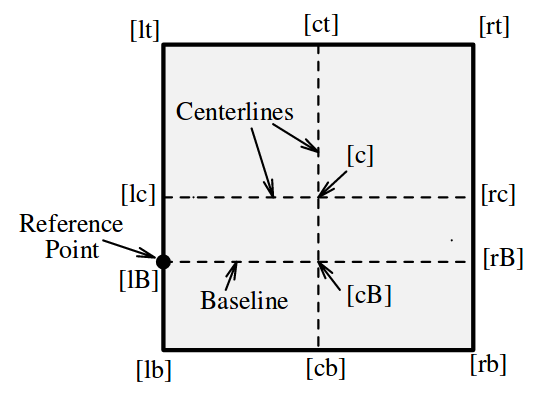
\includegraphics[scale=0.35]{posicoes.png}

\centering
Opções para a chave \textit{origin}: c, lb,rb, \ldots
\end{column}

\begin{column}{6.2cm}
Exemplo:
\begin{lstlisting}[style=latex]

\includegraphics[origin=rb]
                {formas.png}
\end{lstlisting}
\end{column}
\end{columns}
\end{frame}


%%%%%%%%%%%%%%%%%%%%%%%%%%%
\begin{frame}[fragile,t]{Rotação}
\framesubtitle{Opção \textit{origin}}

\makebox[0.65\linewidth][l]{Código \LaTeX:}%
\makebox[0.35\linewidth][l]{Saída:}% 
\vfill
\begin{LTXexample}[style=example,width=0.35\linewidth]

\includegraphics[angle=-180,scale=0.25]
                  {formas.png}

\includegraphics[angle=-180,scale=0.25, 
                 origin=c]{formas.png}
\end{LTXexample}
\end{frame}


%%%%%%%%%%%%%%%%%%%%%%%%%%%
\begin{frame}[fragile,t]{Corte}
\framesubtitle{Opção \textit{trim}}

\begin{columns}
\begin{column}{7cm}
\centering
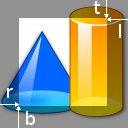
\includegraphics{formas_crop.png}

Opções para a chave \textit{trim}
\end{column}

\begin{column}{7cm}
Exemplo:
\begin{lstlisting}[style=latex]

\includegraphics[trim=r b l t, 
                 clip=true]
                 {formas.png}
\end{lstlisting}
r: direita,
b: base,
l: esquerda,
t: topo.
\end{column}
\end{columns}
\end{frame}

%%%%%%%%%%%%%%%%%%%%%%%%%%%
\begin{frame}[fragile,t]{Corte}
\framesubtitle{Opção \textit{trim}}

\makebox[0.65\linewidth][l]{Código \LaTeX:}%
\makebox[0.35\linewidth][l]{Saída:}% 
\vfill
\begin{LTXexample}[style=example,width=0.35\linewidth]

\includegraphics[scale=0.5]{formas.png}
%
\raisebox{1cm}{$\rightarrow$}
%

\includegraphics[trim=2.45cm 3mm 0 0, 
                   clip=true,
                   scale=0.5]
                   {formas.png}
\end{LTXexample}
\end{frame}

%%%%%%%%%%%%%%%%%%%%%%%%%%%%%%%%%%%%%%%%%%%%%%%%%%%%%%%%%
\section{Legendas}

%%%%%%%%%%%%%%%%%%%%%%%%%%%
\begin{frame}[fragile,t]{Legendas }
\framesubtitle{Comando \textit{figure}}

\makebox[0.65\linewidth][l]{Código \LaTeX:}%
\makebox[0.35\linewidth][l]{Saída:}% 
\vfill
\begin{LTXexample}[style=example,width=0.35\linewidth]
\begin{figure}
  \centering
  
\includegraphics[scale=0.5]{formas.png}
  \caption{Legenda}
\end{figure}
\end{LTXexample}

* Lembre-se de utilizar o idioma correto: 
\begin{lstlisting}[style=latex,linewidth=8cm, xleftmargin=0cm]
\usepackage[brazilian]{babel}
\end{lstlisting}
\end{frame}

%%%%%%%%%%%%%%%%%%%%%%%%%%%
\begin{frame}[fragile,t]{Referência }
\framesubtitle{Comando \textit{label}}

\makebox[0.65\linewidth][l]{Código \LaTeX:}%
\makebox[0.35\linewidth][l]{Saída:}% 
\vfill

\begin{LTXexample}[style=example,width=0.35\linewidth]
Na Figura \ref{fig:formas}, existem 2 formas.

\begin{figure}
  \centering
  
\includegraphics[scale=0.5]{formas.png}
  \caption{Legenda}
  \label{fig:formas}
\end{figure}
\end{LTXexample}

\end{frame}

%%%%%%%%%%%%%%%%%%%%%%%%%%%%%%%%%%%%%%%%%%%%%%%%%%%%%%%%%
\section{Posicionamento}

%%%%%%%%%%%%%%%%%%%%%%%%%%%
\begin{frame}[fragile,t]{Posicionamento}
\framesubtitle{Pacote \textit{float}}

Pacote necessário para o posicionamento de flutuantes: \textit{float}

\begin{lstlisting}[style=latex, linewidth=12cm]
\documentclass{article}

% Pacotes
\usepackage{graphicx}     % figuras
\usepackage{float}        % posicionamento

\begin{document}
  % Inserindo figura posicionada no topo da página
  \begin{figure}[t]
    
\includegraphics{formas.png}
  \end{figure}

\end{document}
\end{lstlisting}
\end{frame}

%%%%%%%%%%%%%%%%%%%%%%%%%%%
\begin{frame}[fragile,t]{Posicionamento}
\framesubtitle{Opções}

Os flutuantes podem ser expostos no topo da página, num lugar específico
ou até em uma página só de figuras. 

\vspace{1cm}

\begin{columns}
\begin{column}{7cm}
\centering
\begin{tabular}{c l}
\hline
\bf Opção & \bf Posição \\
\hline
t     & Parte superior da página   \\
b     & Parte inferior da página   \\
p     & Página de figuras \\
h     & Aqui, se possível \\
H     & Aqui, obrigatoriamente \\
!     & Ignorar sugestão do  \LaTeX\\
\hline
\end{tabular}
\end{column}

\begin{column}{8cm}
Exemplo:
\begin{lstlisting}[style=latex, linewidth=7cm]
\begin{figure}[h]
  \centering
  
\includegraphics{formas.png}
  \caption{Legenda}
\end{figure}
\end{lstlisting}

\end{column}
\end{columns}
\end{frame}

%%%%%%%%%%%%%%%%%%%%%%%%%%%
\begin{frame}[fragile,t]{Posicionamento}
\framesubtitle{Opções \textit{h, t} e \textit{b}}

\begin{columns}
\begin{column}{4.5cm}
\centering
\fbox{\includegraphics[page=1, scale=0.2]{Posicionamento.pdf}}

[h]
\end{column}

\begin{column}{4.5cm}
\centering
\fbox{\includegraphics[page=2, scale=0.2]{Posicionamento.pdf}}

[t]
\end{column}

\begin{column}{4.5cm}
\centering
\fbox{\includegraphics[page=3, scale=0.2]{Posicionamento.pdf}}

[b]
\end{column}
\end{columns}
\end{frame}

%%%%%%%%%%%%%%%%%%%%%%%%%%%
\begin{frame}[fragile,t]{Posicionamento}
\framesubtitle{Opção \textit{H}}

\begin{columns}
\begin{column}{0cm}
[H]
\end{column}

\begin{column}{4cm}
\centering
\fbox{\includegraphics[page=4, scale=0.2]{Posicionamento.pdf}}

Página 1
\end{column}

\begin{column}{4cm}
\centering
\fbox{\includegraphics[page=5, scale=0.2]{Posicionamento.pdf}}

Página 2
\end{column}
\end{columns}

\end{frame}

%%%%%%%%%%%%%%%%%%%%%%%%%%%
\begin{frame}[fragile,t]{Posicionamento}
\framesubtitle{Opção \textit{h}}

\begin{columns}
\begin{column}{0cm}
[h]
\end{column}

\begin{column}{4cm}
\centering
\fbox{\includegraphics[page=6, scale=0.2]{Posicionamento.pdf}}

Página 1
\end{column}

\begin{column}{4cm}
\centering
\fbox{\includegraphics[page=7, scale=0.2]{Posicionamento.pdf}}

Página 2
\end{column}
\end{columns}

\end{frame}

%%%%%%%%%%%%%%%%%%%%%%%%%%%
\begin{frame}[fragile,t]{Posicionamento}
\framesubtitle{Opção \textit{p}}

\begin{columns}
\begin{column}{0cm}
[p]
\end{column}

\begin{column}{4cm}
\centering
\fbox{\includegraphics[page=8, scale=0.2]{Posicionamento.pdf}}

Página 1
\end{column}

\begin{column}{4cm}
\centering
\fbox{\includegraphics[page=9, scale=0.2]{Posicionamento.pdf}}

Página 2
\end{column}
\end{columns}

\end{frame}

%%%%%%%%%%%%%%%%%%%%%%%%%%%%%%%%%%%%%%%%%%%%%%%%%%%%%%%%%
\section{Subfiguras}

%%%%%%%%%%%%%%%%%%%%%%%%%%%
\begin{frame}[fragile,t]{Subfiguras}
\framesubtitle{Pacote \textit{subfigure}}

Pacote necessário para o uso de subfiguras: \textit{subfigure}

\begin{lstlisting}[style=latex, linewidth=12cm]
\documentclass{article}
% Pacotes
\usepackage{graphicx}       % figuras
\usepackage{subfigure}      % subfiguras

\begin{document}
  % Inserindo subfiguras 
  \begin{figure}
    \subfigure{\includegraphics{fig1.png}}
    \subfigure{\includegraphics{fig2.png}}
    \caption{Legenda}
  \end{figure}
\end{document}
\end{lstlisting}
\end{frame}

%%%%%%%%%%%%%%%%%%%%%%%%%%%
\begin{frame}[fragile,t]{Subfiguras}
\framesubtitle{Comando \textit{subfigure}}

\makebox[0.65\linewidth][l]{Código \LaTeX:}%
\makebox[0.35\linewidth][l]{Saída:}% 
\vfill

\begin{LTXexample}[style=example,width=0.35\linewidth]
\begin{figure}
  \centering
  \subfigure{
    
\includegraphics[scale=0.4]{formas.png}%
  }
  \hspace{0.5cm}
  \subfigure{
    
\includegraphics[scale=0.4]{formas.png}%
  }
  \caption{Subfiguras}
 \end{figure}
\end{LTXexample}

\end{frame}

%%%%%%%%%%%%%%%%%%%%%%%%%%%
\begin{frame}[fragile,t]{Subfiguras Legendadas}
\framesubtitle{Opção [\textit{Legenda}]}

\makebox[0.65\linewidth][l]{Código \LaTeX:}%
\makebox[0.35\linewidth][l]{Saída:}% 
\vfill

\begin{LTXexample}[style=example,width=0.35\linewidth]
\begin{figure}
  \centering
  \subfigure[Legenda 1]{
    
\includegraphics[scale=0.4]{formas.png}%
  }
  \hspace{0.5cm}
  \subfigure[Legenda 2]{
    
\includegraphics[scale=0.4]{formas.png}%
  }
  \caption{Subfiguras}
 \end{figure}
\end{LTXexample}

\end{frame}

%%%%%%%%%%%%%%%%%%%%%%%%%%%
\begin{frame}[fragile,t]{Subfiguras Referenciáveis}
\framesubtitle{Opção [ ]}

\makebox[0.65\linewidth][l]{Código \LaTeX:}%
\makebox[0.35\linewidth][l]{Saída:}% 
\vfill

\begin{LTXexample}[style=example,width=0.35\linewidth]
\begin{figure}
  \centering
  \subfigure[]{\label{fig:formas-a}
    
\includegraphics[scale=0.4]{formas.png}%
  }
  \hspace{0.5cm}
  \subfigure[]{\label{fig:formas-b}
    
\includegraphics[scale=0.4]{formas.png}%
  }
  \caption{Subfiguras}
 \end{figure}
\end{LTXexample}

\end{frame}

%%%%%%%%%%%%%%%%%%%%%%%%%%%
\begin{frame}[fragile,t]{Subfiguras}
\framesubtitle{Inclusão com opção \textit{FIGTOPCAP}}

É possível posicionar as legendas das subfiguras acima das mesmas,
adicionando o parâmetro \textit{FIGTOPCAP} ao incluir o pacote:

\begin{lstlisting}[style=latex,linewidth=11cm, xleftmargin=0cm]
\usepackage[FIGTOPCAP]{subfigure}
\end{lstlisting}

\begin{figure}
  \centering
  \subfiguretopcaptrue
  \subfigure[]{
\includegraphics[scale=0.4]{formas.png}}
  \hspace{1cm}
  \subfigure[]{
\includegraphics[scale=0.4]{formas.png}}
  \caption{Subfiguras}
 \end{figure}

\end{frame}

%%%%%%%%%%%%%%%%%%%%%%%%%%%
\begin{frame}[fragile,t]{Subfiguras}
\framesubtitle{Inclusão com opção \textit{FIGTOPCAP} e \textit{nooneline}}

É possível posicionar as legendas das subfiguras acima das mesmas no canto
direito, adicionando 2 parâmetros ao incluir o pacote:

\begin{lstlisting}[style=latex,linewidth=11cm, xleftmargin=0cm]
\usepackage[FIGTOPCAP,nooneline]{subfigure}
\end{lstlisting}

\begin{figure}
  \centering
  \subfiguretopcaptrue
  \subcapnoonelinetrue
  \subfigure[]{
\includegraphics[scale=0.4]{formas.png}}
  \hspace{1cm}
  \subfigure[]{
\includegraphics[scale=0.4]{formas.png}}
  \caption{Subfiguras}
 \end{figure}

\end{frame}

%%%%%%%%%%%%%%%%%%%%%%%%%%%%%%%%%%%%%%%%%%%%%%%%%%%%%%%%%
\section{Pasta de Figuras}

%%%%%%%%%%%%%%%%%%%%%%%%%%%
\begin{frame}[fragile,t]{Pasta de figuras}
\framesubtitle{Comando \textit{graphicspath}}

É possível especificar uma pasta de figuras.

\begin{lstlisting}[style=latex, linewidth=12cm]
\documentclass{article}
% Pacotes
\usepackage{graphicx}       % figuras
\graphicspath{{./figs/}}    % pasta de figuras

\begin{document}
  \begin{figure}
    % Figura localizada em ./figs
    \includegraphics{fig1.png}
    \caption{Legenda}
  \end{figure}
\end{document}
\end{lstlisting}
\end{frame}

%%%%%%%%%%%%%%%%%%%%%%%%%%%
\begin{frame}[fragile,t]{Pastas de figuras}
\framesubtitle{Comando \textit{graphicspath}}

É possível especificar mais de uma pasta de figuras.

\begin{lstlisting}[style=latex, linewidth=12cm]
\documentclass{article}
% Pacotes
\usepackage{graphicx}              % figuras
\graphicspath{{./figs/}{../figs/}} % pastas de figuras

\begin{document}
  \begin{figure}
    % Figura localizada em ./figs ou ../figs
    \includegraphics{fig1.png}
    \caption{Legenda}
  \end{figure}
\end{document}
\end{lstlisting}
\end{frame}

%%%%%%%%%%%%%%%%%%%%%%%%%%%%%%%%%%%%%%%%%%%%%%%%%%%%%%%%%
\section{Formatos de Imagem}

%%%%%%%%%%%%%%%%%%%%%%%%%%%
\begin{frame}[fragile,t]{Tipos de Imagem}
\framesubtitle{Imagem em pixels vs vetorizada}

\vspace{0.5cm}
\centering
 \begin{tabular}{p{5cm}p{5cm}}
 
\includegraphics[width=4.5cm]{figura.pdf} &
 
\includegraphics[width=4.5cm]{figura_200_dpi.png} \\
 \\
 (a) Imagem vetorizada      &  (b) Imagem em pixels \\
  \qquad(eps, pdf, svg)     & \qquad(png, jpeg, gif)  \\
 \end{tabular}
 \vspace{1cm}

A principal diferença é a perda de definição ao ampliarmos a imagem.
\end{frame}

%%%%%%%%%%%%%%%%%%%%%%%%%%%
\begin{frame}[fragile,t]{Imagens Vetorizadas}
\framesubtitle{Formatos}

Os principais formatos de imagens vetorizadas suportados pelo \LaTeX \ são:

\vspace{0.5cm}
\centering
 \begin{tabular}{p{5cm}p{5cm}}
 
\includegraphics[width=4.5cm]{figura.pdf} & 
 \includegraphics[width=4.5cm]{figura.eps} \\
 \\
 (a) Formato pdf (5,5 kb) &  (b) Formato eps (11,8 kb)\\
 \end{tabular}

\end{frame}

%%%%%%%%%%%%%%%%%%%%%%%%%%%
\begin{frame}[fragile,t]{Imagens Vetorizadas}
\framesubtitle{Formato svg}

Arquivos no formato svg podem ser editados e gerar diversos formatos, como pdf, eps, png e jpg.

\vspace{1cm}
\centering
\includegraphics[width=10cm]{formatos.pdf}

\end{frame}

%%%%%%%%%%%%%%%%%%%%%%%%%%%
\begin{frame}[fragile,t]{Imagens Vetorizadas}
\framesubtitle{Editores de imagem}

Alguns editores de imagens vetorizadas são:

\vspace{1cm}
\centering
\begin{tabular}{p{3cm}p{3cm}p{3cm}p{3cm}}
\href{http://coreldraw.com}{\includegraphics[width=2cm]{coreldraw.png}} &
\href{http://inkscape.org }{\includegraphics[width=2cm]{inkscape.png}} &
\href{http://gimp.org     }{\includegraphics[width=2cm]{gimp.png}} &
\href{http://vectr.com    }{\includegraphics[width=2cm]{vectr.png}} \\
\\
(a) CorelDRAW  &  (b) Inkscape  &  (c) Gimp   &  (d) Vectr \\
\end{tabular}

\end{frame}

%%%%%%%%%%%%%%%%%%%%%%%%%%%
\begin{frame}[fragile,t]{Imagens em Pixels}
\framesubtitle{Formatos}

Os principais formatos de imagens em pixels suportados pelo \LaTeX  \ são:

\vspace{0.5cm}
\centering
\begin{tabular}{p{5cm}p{5cm}}
 \includegraphics[width=4.5cm]{figura_200_dpi.png} &
 \includegraphics[width=4.5cm]{figura_200_dpi_q100.jpg} \\
 \\
 (a) Formato png  &  (b) Formato jpg \\
 \end{tabular}

\end{frame}

%%%%%%%%%%%%%%%%%%%%%%%%%%%
\begin{frame}[fragile,t]{Imagens em Pixels}
\framesubtitle{Formato png}

\textbf{Formato png}: Ideal para ilustrações. Formato com maior qualidade.

\vspace{1cm}
\centering
 \begin{tabular}{p{4.5cm}p{4.5cm}p{4.5cm}}
 \includegraphics[width=4cm]{figura_400_dpi.png} & 
 \includegraphics[width=4cm]{figura_200_dpi.png} &
 \includegraphics[width=4cm]{figura_100_dpi.png} \\
 \\
 (a) 400 dpi (18,9 kb)  &  (b) 200 dpi (8,9 kb)  & (c) 100 dpi (4,4 kb)\\

 \end{tabular}

\end{frame}

%%%%%%%%%%%%%%%%%%%%%%%%%%%
\begin{frame}[fragile,t]{Imagens em Pixels}
\framesubtitle{Formato jpg}

\textbf{Formato jpg}: Ideal para fotos. Formato mais compacto quanto menor a qualidade.

\vspace{1cm}
\centering
 \begin{tabular}{p{4.5cm}p{4.5cm}p{4.5cm}}
 \includegraphics[width=4cm]{figura_200_dpi_q100.jpg} & 
 \includegraphics[width=4cm]{figura_200_dpi_q050.jpg} &
 \includegraphics[width=4cm]{figura_200_dpi_q010.jpg} \\
 \\
 (a) Qualidade 100\%  &  (b) Qualidade 50\%  & (c) Qualidade 10\%\\
 \qquad (15,3 kb)     & \qquad (4,4 kb)      & \qquad (2,3 kb)
 \end{tabular}

\end{frame}

%%%%%%%%%%%%%%%%%%%%%%%%%%%
\begin{frame}[fragile,t]{Imagens em Pixels}
\framesubtitle{Editores de imagem}

Alguns editores de imagens em pixels são:

\vspace{1cm}
\centering
\begin{tabular}{p{3cm}p{3cm}p{3cm}p{3cm}}
\href{http://photoshop.com}{\includegraphics[width=2cm]{ps.jpeg}} &
\href{http://getpaint.net }{\includegraphics[width=2cm]{paintnet.jpg}} &
\href{http://gimp.org     }{\includegraphics[width=2cm]{gimp.png}} &
\href{http://pixlr.com    }{\includegraphics[width=2cm]{pixlr.png}} \\
\\
(a) Photoshop  &  (b) Paint.net  &  (c) Gimp &  (d) Pixlr \\
\end{tabular}

\end{frame}

%%%%%%%%%%%%%%%%%%%%%%%%%%%
\begin{frame}[fragile,t]{Extensão das figuras}
% \framesubtitle{Comando \textit{DeclareGraphicsExtensions}}

É possível omitir a extensão das figuras. O \LaTeX \ procura
pela extensão existente.

\begin{lstlisting}[style=latex, linewidth=12cm]
\documentclass{article}
% Pacotes
\usepackage{graphicx}            % figuras

\begin{document}
  \begin{figure}
    \includegraphics{fig1}       % Inclui fig1.png
    \includegraphics{fig2}       % Inclui fig2.pdf
    \caption{Legenda}
  \end{figure}
\end{document}
\end{lstlisting}
\end{frame}

%%%%%%%%%%%%%%%%%%%%%%%%%%%
\begin{frame}[fragile,t]{Extensão das figuras}
\framesubtitle{Comando \textit{DeclareGraphicsExtensions}}

Se existir mais de uma extensão admissível, é possível definir
a ordem de busca com o comando \textit{DeclareGraphicsExtensions}.

\begin{lstlisting}[style=latex, linewidth=12cm]
\documentclass{article}
\usepackage{graphicx}         

% Busca pela extensão png, depois por pdf   
\DeclareGraphicsExtensions{.png, .pdf}

\begin{document}
  \begin{figure}
    \includegraphics{fig1}      % Inclui fig1.pdf
    \caption{Legenda}
  \end{figure}
\end{document}
\end{lstlisting}
\end{frame}

\end{document}
